\documentclass{article}
\usepackage[utf8]{inputenc}
\title{Early Detection of Interest Loss in Hebrew WhatsApp Sales Conversations: Textual, Behavioral, and Prefix-Aware Modeling}
\author{Roni Twito (ID. 313221467), Matan Zohar Cohen (ID. 209225457)}
\date{Submitted as final project report for the NLP course, Reichman University, 2026}
\usepackage{natbib}
\usepackage{graphicx}
\usepackage{booktabs}
\usepackage{array}
\usepackage{amsmath}
\usepackage{hyperref}
\usepackage{enumitem}
\usepackage{subcaption}
\setlist[enumerate]{itemsep=1pt,parsep=1pt,topsep=3pt}
\renewcommand{\textfraction}{0.1}
\renewcommand{\topfraction}{0.9}
\renewcommand{\bottomfraction}{0.9}
\renewcommand{\floatpagefraction}{0.7}
\setcounter{topnumber}{4}
\setcounter{bottomnumber}{4}
\setcounter{totalnumber}{6}
\begin{document}
\maketitle

\begin{abstract}
Loss of customer interest can surface not only in what participants say but in how communication behavior changes over time. We study early detection of interest loss in Hebrew WhatsApp sales conversations as binary classification (\texttt{interested} vs.\ \texttt{losing\_interest}) over a synthetic, LLM-generated dataset of 3,055 conversations (2,137/459/459 train/validation/test, class-balanced, conversation-level split, seed 42). We compare behavioral, lexical, and semantic (AlephBERT) representations on complete conversations, then evaluate prediction quality at partial observation points (25/50/75/100\%). A model fine-tuned only on complete conversations degrades sharply on partial conversations (macro-F1 33.28/33.77/51.14\% at 25/50/75\%), motivating prefix-aware training, which raises early-stage macro-F1 to 62.64/74.84/86.93\% at a modest cost to full-conversation performance (95.20\% vs.\ 98.04\%). Adding 26 non-lexical behavioral features to the prefix-aware model yields directional gains, most notably at 75\% ($+2.18$ pp, bootstrap 95\% CI $[+0.20, +4.36]$), but McNemar tests reach no significance at any prefix (all $p>0.05$), and the effect reverses at 100\% ($-0.88$ pp). A controlled ablation shows the apparent full-conversation gain from behavioral fusion (97.38\% vs.\ 96.95\%) is better explained by additional training than behavioral information: a text-only continued-training control reaches 98.04\%. Our results support a nuanced conclusion: behavioral dynamics carry standalone predictive signal, prefix-aware training is essential for early detection, and behavioral fusion provides directional but not conclusively significant value when text is incomplete.
\end{abstract}

\section{Introduction}

Interest loss in a sales conversation is typically framed as a text-classification problem: given what a customer says, predict whether they remain interested. This overlooks a second evidence source: communication-behavior change over a conversation -- response latency, message length, participation balance -- may signal disengagement even when text is ambiguous. A more important limitation: standard framings classify complete conversations, whereas a business needs to detect interest loss while a conversation is still ongoing, so intervention remains possible. We therefore study early detection of interest loss as binary classification (\texttt{interested} vs.\ \texttt{losing\_interest}), evaluated both on complete conversations and on prefixes representing 25\%, 50\%, and 75\% of observed messages.

\subsection{Related Work}
\label{sec:relwork}

We build on AlephBERT \citep{Seker2022} as a fixed architecture (HeRo \citep{Shalumov2023} is untested). Related early-detection work includes earliness/accuracy surveys \citep{Renault2024}; sequential-reading text classification \citep{DulacArnold2011}; conversation-derailment forecasting \citep{Chang2019}; rumor and depression-risk detection from partial social-media streams \citep{Song2019,Burdisso2019}; early-observation sufficiency for churn prediction \citep{Han2026}; engagement/failure prediction combining behavioral and textual signals \citep{Meng2021,Nourbakhsh2026}; and behavioral-only churn prediction \citep{Mufti2026}. Unlike this prior work, we run a controlled ablation (Section~\ref{sec:ablation}) and paired bootstrap/McNemar testing (Section~\ref{sec:statval}) before attributing gains to behavioral information.

\subsection{Research Questions and Contributions}
\label{sec:rq}

\noindent\textbf{RQ1.} How effectively can textual and behavioral signals classify interest state in complete Hebrew WhatsApp conversations? \textbf{RQ2.} Does a model trained only on complete conversations generalize to early prediction from partial (prefix) conversations? \textbf{RQ3.} Does prefix-aware training -- explicitly training on conversation prefixes -- improve early detection relative to a full-conversation-trained model evaluated on prefixes? \textbf{RQ4.} Do explicit, non-lexical behavioral signals provide additional predictive value beyond a prefix-aware AlephBERT model when textual evidence is incomplete?

Full-conversation classification (Sections~\ref{sec:fullconv}--\ref{sec:ablation}, RQ1) measures a representational ceiling, while prefix-based early detection (Sections~\ref{sec:e1}--\ref{sec:statval}, RQ2--RQ4) measures detectability while a conversation is still actionable.

This work's contribution is primarily problem framing, methodology, and careful interpretation, not new model architecture: (1) framing interest-loss detection as early, not only full-conversation, prediction; (2) evaluating prediction quality at four observation points (25/50/75/100\%); (3) comparing full-conversation training against prefix-aware training under an identical architecture; (4) testing whether behavioral dynamics add value beyond text when evidence is incomplete, via (5) a controlled ablation isolating a training-duration confound, (6) paired bootstrap/McNemar validation, and (7) decomposing the E2-vs-E3 comparison by true class (Section~\ref{sec:classlevel}), showing an aggregate gain can mask a class-asymmetric pattern.

\section{Methodology}
\label{sec:methodology}

\subsection{Dataset and Task Definition}
\label{sec:dataset}

Given a chronologically ordered WhatsApp sales conversation (interleaved customer/business turns), the task predicts a binary label, \texttt{interested} or \texttt{losing\_interest}, from the complete conversation or a prefix of its first 25\%, 50\%, or 75\% of messages. The dataset is entirely synthetic, including the original 300-conversation seed, itself synthetically generated and then used to seed further LLM-based generation (GPT-4o-mini/GPT-4o/GPT-5-mini); no real WhatsApp or customer data were used, and every record is flagged \texttt{synthetic: true} (Section~\ref{sec:limitations}). It contains 3,055 conversations, split 2,137/459/459 (train/val/test, $\approx$70/15/15), stratified by label at the conversation level (seed 42). Classes are close to balanced: 1,529 \texttt{interested} (50.05\%) and 1,526 \texttt{losing\_interest} (49.95\%). We report macro-F1 throughout.

\subsection{Textual Representation}
\label{sec:textrep}

We use AlephBERT (\texttt{onlplab/alephbert-base}; \citealp{Seker2022}), a Hebrew pretrained transformer, fine-tuned with a classification head (max sequence length 512 tokens, truncation).

\subsection{Behavioral and Lexical Features}
\label{sec:behavioral}

We compute 26 pure, non-lexical behavioral features from conversation structure and timing metadata, in six groups: participation/message counts, customer message-length statistics, response timing, session/gap structure, conversation-ending structure, and temporal change (first- vs.\ second-half differences). A separate handcrafted lexical feature set (25 features: question/emoji rates, Hebrew price/negotiation/objection/commitment/delay-signal keywords, positional presence) is used only in the Behavioral+Lexical baseline (Table~\ref{tab:table1}); see the table caption for the feature-count breakdown.

\subsection{Prefix Construction and Leakage Prevention}
\label{sec:prefix}

For a conversation with $N$ messages, the $k\%$ prefix retains the first $\max(1, \lceil N \times k \rceil)$ messages; text and behavioral features are recomputed from only those messages, so no future information leaks into any prefix -- enforced and unit-tested.

\subsection{Prefix-Aware Training and Fusion}
\label{sec:training}

Prefix-aware models (E2, E3) augment each training conversation into all four prefix fractions (25/50/75/100\%), directly optimizing the model to classify from partial evidence. In fusion models, standardized behavioral features are concatenated with the AlephBERT representation and passed through a small MLP head (hidden dim.\ 256, dropout 0.1); E3's encoder and head use separate learning rates ($1\times10^{-5}$ and $1\times10^{-3}$), mirroring the continued-training control (Section~\ref{sec:ablation}).

\subsection{Implementation, Training, and Evaluation Details}
\label{sec:implementation}

Full-conversation models select the checkpoint with the best validation macro-F1; prefix-aware models (E2, E3) select the checkpoint maximizing average macro-F1 across the 25/50/75\% validation prefixes (excluding 100\%) to favor early-detection quality. We report macro-F1 (primary), accuracy, per-class precision/recall/F1, and weighted-F1. For RQ4, we run a paired bootstrap (10,000 resamples, 95\% CI) and a paired McNemar exact test at each prefix; seed 42 throughout.

\section{Experimental Results}
\label{sec:results}

\subsection{Experimental Setup}
\label{sec:setup}

AlephBERT fine-tuning uses 5 epochs, learning rate $2\times10^{-5}$, weight decay 0.01, warmup ratio 0.1, gradient clipping 1.0, batch size 8 (train) / 16--32 (eval). Behavioral-only baselines compare logistic regression and a random forest (200 trees); the random forest performs better and is reported.

\subsection{Full-Conversation Classification (RQ1)}
\label{sec:fullconv}

Table~\ref{tab:table1} compares five full-conversation models. The pure behavioral baseline (26 features, random forest) reaches 65.07\% macro-F1, well above a degenerate single-class predictor ($\sim$33\%). Adding lexical cues (43 features) raises macro-F1 to 86.69\%, and AlephBERT text-only reaches 96.95\% -- answering RQ1: text alone is already highly effective, while behavioral signal is real but weaker and complementary.

\begin{table}[htbp]
\centering
\small
\begin{tabular}{@{}p{3.1cm}p{3.6cm}p{1.6cm}c@{}}
\toprule
Model & Features & Feat.\ count & Test Macro-F1 \\
\midrule
Pure Behavioral & Non-lexical behavioral only & 26 & 65.07\% \\
Behavioral + Lexical & Structural + lexical keyword & 43* & 86.69\% \\
AlephBERT (text-only) & Full conversation text & -- & 96.95\% \\
AlephBERT + Behavioral Fusion & Text + 26 behavioral & 26+text & 97.38\% \\
AlephBERT, continued training (control) & Text only, same extra training as Fusion & -- & 98.04\% \\
\bottomrule
\end{tabular}
\caption{Full-conversation model comparison ($n=459$). *43 = 18 structural + 25 lexical, predating the 8 temporal-change features (Section~\ref{sec:behavioral}).}
\label{tab:table1}
\end{table}

\subsection{Controlled Continued-Training Ablation}
\label{sec:ablation}

Fusing AlephBERT with the 26 behavioral features reaches 97.38\% macro-F1, a nominal improvement over the 96.95\% text-only baseline (Table~\ref{tab:table1}). However, fusion also involves extra fine-tuning steps beyond the original checkpoint, so this alone cannot separate behavioral information from training duration. A continued-training control -- same extra steps, no behavioral features -- reaches 98.04\% macro-F1, higher than the fusion model, since the apparent gain cannot be attributed to behavioral features when an equivalently-trained text-only model outperforms it.

\subsection{E1: Full-Conversation Model on Prefixes (RQ2)}
\label{sec:e1}

We evaluated the continued-training AlephBERT model (98.04\% full-conversation), without retraining, on test-conversation prefixes (E1). Performance collapses at early stages: 33.28\% macro-F1 at 25\%, 33.77\% at 50\%, and 51.14\% at 75\% (Table~\ref{tab:table2}, Figure~\ref{fig:combined}a), answering RQ2: a full-conversation-trained model does not generalize to partial conversations.

\subsection{E2: Prefix-Aware AlephBERT (RQ3)}
\label{sec:e2}

Training the identical architecture with prefix augmentation (E2) improves early detection: macro-F1 rises to 62.64\% (25\%), 74.84\% (50\%), and 86.93\% (75\%), reaching 95.20\% at 100\% (Table~\ref{tab:table2}, Figure~\ref{fig:combined}a). This answers RQ3: prefix-aware training is necessary and effective for early detection at modest full-conversation cost.

\subsection{E3: Prefix-Aware Behavioral Fusion (RQ4)}
\label{sec:e3}

E3 adds the same 26 behavioral features, computed leakage-safe per prefix, to the prefix-aware model. Point-estimate macro-F1 (Table~\ref{tab:table2}): 64.45\% at 25\%, 74.92\% at 50\%, 89.11\% at 75\%, and 94.32\% at 100\%. The largest gain over E2 appears at 75\% observation (Table~\ref{tab:table3}).

\begin{table}[htbp]
\centering
\small
\begin{tabular}{@{}cccc@{}}
\toprule
Prefix & E1 (full-conv.\ on prefixes) & E2 (prefix-aware) & E3 (prefix-aware + behavioral) \\
\midrule
25\%  & 33.28\% & 62.64\% & 64.45\% \\
50\%  & 33.77\% & 74.84\% & 74.92\% \\
75\%  & 51.14\% & 86.93\% & 89.11\% \\
100\% & 98.04\% & 95.20\% & 94.32\% \\
\bottomrule
\end{tabular}
\caption{Macro-F1 (\%) by conversation prefix: E1, E2, E3.}
\label{tab:table2}
\end{table}

\subsection{Statistical Validation of E2 vs.\ E3}
\label{sec:statval}

A paired bootstrap and McNemar test (Table~\ref{tab:table3}) assess whether the E3 gains (Section~\ref{sec:e3}) are reliable. Only the 75\% CI excludes zero ($[+0.20, +4.36]$ pp); no McNemar $p$-value reaches $\alpha=0.05$, though 75\% comes closest ($p=0.0639$; E3 corrects 17, introduces 7 errors, net +10/459). We therefore do not claim behavioral features significantly improve early detection at this test-set size; the evidence is directional, strongest at 75\%, and reverses at 100\%, answering RQ4: fusion gives modest, direction-consistent but not conclusively significant value when text is incomplete.

\begin{table}[htbp]
\centering
\small
\begin{tabular}{@{}cccccc@{}}
\toprule
Prefix & $\Delta$ E3$-$E2 (pp) & 95\% Bootstrap CI (pp) & McNemar $p$ & Fixes/Regr.\ & Net \\
\midrule
25\%  & +1.82 & [$-2.02$, +5.88] & 0.5052 & 44/37 & +7 \\
50\%  & +0.08 & [$-2.94$, +3.01] & 1.0000 & 23/23 & 0 \\
75\%  & +2.18 & [+0.20, +4.36]   & 0.0639 & 17/7  & +10 \\
100\% & $-0.88$ & [$-1.98$, 0.00] & 0.2188 & 1/5   & $-4$ \\
\bottomrule
\end{tabular}
\caption{Paired bootstrap and McNemar statistics for E2 vs.\ E3 ($n=459$), with per-prefix error counts.}
\label{tab:table3}
\end{table}

\begin{figure}[htbp]
\centering
\begin{subfigure}[b]{0.48\textwidth}
\centering
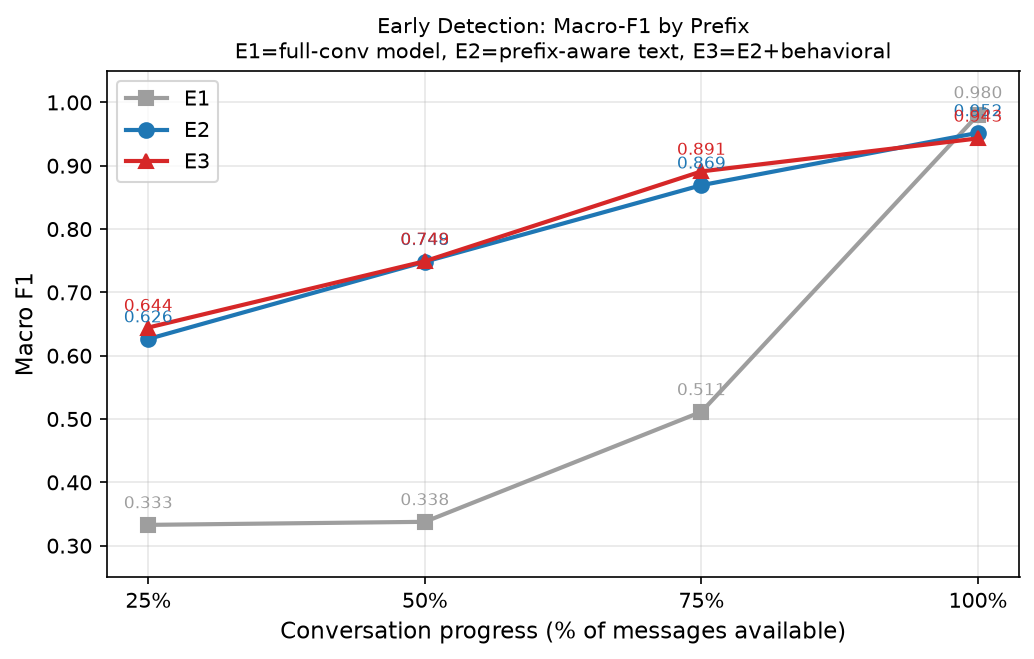
\includegraphics[width=\textwidth]{figures/fig1_macro_f1_by_prefix.png}
\caption{Macro-F1 vs.\ prefix, E1/E2/E3.}
\label{fig:fig1}
\end{subfigure}
\hfill
\begin{subfigure}[b]{0.48\textwidth}
\centering
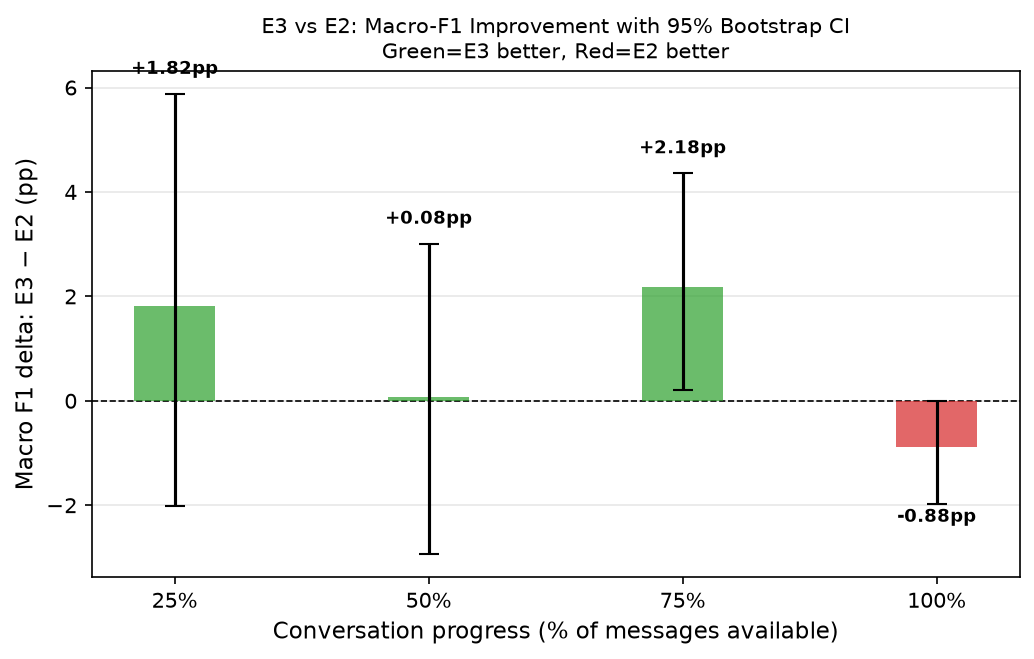
\includegraphics[width=\textwidth]{figures/fig2_delta_with_ci.png}
\caption{E3$-$E2 delta with 95\% CI.}
\label{fig:fig2}
\end{subfigure}
\caption{Early-detection performance by conversation prefix.}
\label{fig:combined}
\end{figure}

\subsection{Class-Level Error Analysis}
\label{sec:classlevel}

Table~\ref{tab:table4} breaks the E3-vs-E2 comparison by true label: net gains are not evenly distributed. E3 is net-positive on truly \texttt{interested} conversations at every non-100\% prefix, but net-negative on truly \texttt{losing\_interest} conversations at every prefix. The aggregate macro-F1 gain is driven mostly by fixing false \texttt{losing\_interest} predictions on \texttt{interested} conversations, while disengaging conversations see more new errors than fixes. E3 is also usually more confident than E2 on its own new errors: at 75\%, mean confidence on E3's regressions is 0.995 vs.\ E2's 0.749, and \texttt{losing\_interest} regressions reach 0.94--1.00 mean E3 confidence at every prefix.

\begin{table}[htbp]
\centering
\small
\begin{tabular}{@{}ccc@{}}
\toprule
Prefix & Net (true = \texttt{interested}) & Net (true = \texttt{losing\_interest}) \\
\midrule
25\%  & +18 (32 fixes / 14 regr.) & $-11$ (12 fixes / 23 regr.) \\
50\%  & +7 (17 fixes / 10 regr.)  & $-7$ (6 fixes / 13 regr.) \\
75\%  & +11 (14 fixes / 3 regr.) & $-1$ (3 fixes / 4 regr.) \\
100\% & 0 (0 fixes / 0 regr.)    & $-4$ (1 fixes / 5 regr.) \\
\bottomrule
\end{tabular}
\caption{E3 vs.\ E2 net outcome (fixes minus regressions) by true class and prefix ($n=459$; 230 interested, 229 losing\_interest).}
\label{tab:table4}
\end{table}

\section{Discussion}
\label{sec:discussion}

\subsection{Main Findings}

AlephBERT dominates on complete conversations and fusion adds nothing attributable to behavioral content (Section~\ref{sec:ablation}); behavioral information matters most at 75\%, but the test set lacks power beyond a directional trend, and the gain concentrates on one class (Section~\ref{sec:classlevel}).

\subsection{Limitations}
\label{sec:limitations}

\begin{enumerate}
\item The 459-conversation test set limits statistical power, especially per-prefix (E2/E3 disagreement as low as 23--61 conversations); a larger test set is needed to confirm the 75\% effect.
\item The dataset is entirely synthetic (including the 300-conversation seed), strictly binary, and specific to Hebrew sales conversations, and models used a single seed (split, classical models, bootstrap fix seed 42); results may not transfer to authentic data or generalize to intermediate engagement, other languages, or domains; multi-seed replication is future work.
\item The E3 gains are class-asymmetric (Section~\ref{sec:classlevel}): driven mostly by correcting false \texttt{losing\_interest} predictions on interested conversations, while net-negative on truly \texttt{losing\_interest} conversations at every prefix, invisible in Table~\ref{tab:table2}.
\end{enumerate}

\subsection{Conclusion / Final Takeaways}
\label{sec:conclusion}

\textbf{RQ1--RQ4} are answered in Sections~\ref{sec:fullconv}--\ref{sec:statval}: text alone is highly effective on complete conversations; a full-conversation-trained model does not generalize to partial ones; prefix-aware training is necessary at modest cost; and behavioral fusion gives directional, class-asymmetric, but not conclusively significant value when text is incomplete.

\section{Code}

Code and experiment scripts:\\
\url{https://github.com/ZoharCohenDev/whatsapp-emotion-analysis}

\bibliographystyle{plain}
\bibliography{references}

\end{document}
